\begin{figure}[htbp]
	\centering
	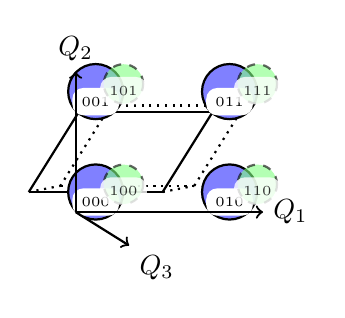
\begin{tikzpicture}[scale=0.85]
		\def\ax{2}
		\def\ay{1.5}
		\def\az{1.2}
		
	\begin{scope}[cm={1,0,0.5,0.8,(-1cm,0cm)}]
		% Front face edges (SOLID)
		\draw[thick] (0,0,0) -- (2,0,0);
		\draw[thick] (2,0,0) -- (2,1.5,0);
		\draw[thick] (2,1.5,0) -- (0,1.5,0);
		\draw[thick] (0,1.5,0) -- (0,0,0);
		
		% Back face edges (DOTTED)
		\draw[dotted, thick] (0.8,0.5,1) -- (2.8,0.5,1);
		\draw[dotted, thick] (2.8,0.5,1) -- (2.8,2,1);
		\draw[dotted, thick] (2.8,2,1) -- (0.8,2,1);
		\draw[dotted, thick] (0.8,2,1) -- (0.8,0.5,1);
		
		% Connecting lines front-to-back (DOTTED, 4 lines)
		\draw[dotted, thick] (0,0,0) -- (0.8,0.5,1);
		\draw[dotted, thick] (2,0,0) -- (2.8,0.5,1);
		\draw[dotted, thick] (0,1.5,0) -- (0.8,2,1);
		\draw[dotted, thick] (2,1.5,0) -- (2.8,2,1);
	\end{scope}
		
		\foreach \x/\y/\z/\label in {0/0/0/000, 2/0/0/010, 0/1.5/0/001, 2/1.5/0/011} {
			\node[draw, circle, fill=blue!50, minimum size=0.7cm, thick] at (\x,\y,\z) {};
			\node[fill=white, rounded corners, font=\tiny] at (\x,\y-0.15,\z) {\label};
		}
		
		\foreach \x/\y/\z/\label in {0.8/0.5/1/100, 2.8/0.5/1/110, 0.8/2/1/101, 2.8/2/1/111} {
			\node[draw, circle, fill=green!50, minimum size=0.5cm, thick, dashed, opacity=0.6] at (\x,\y,\z) {};
			\node[fill=white, opacity=0.8, rounded corners, font=\tiny] at (\x,\y-0.1,\z) {\label};
		}
		
		\draw[->, thick] (-0.3,-0.3) -- (2.5,-0.3) node[right] {$Q_1$};
		\draw[->, thick] (-0.3,-0.3) -- (-0.3,1.8) node[above] {$Q_2$};
		\draw[->, thick] (-0.3,-0.3) -- (0.5,-0.8) node[below right] {$Q_3$};
		
	\end{tikzpicture}
	\caption{Three-qubit state in Dimensional Circular Notation, shown in isometric projection. The cube structure represents the three-dimensional arrangement corresponding to three qubits.}
	\label{fig:dcn-3qubit}
\end{figure}
